\section{Introduction}
\label{sec:introduction}

Speech is the most natural channel of human communication, and Speech
Large Language Models (Speech LLMs) are now closing the gap between
text-based language modeling and real-time spoken interaction
\cite{chen2023salmspeechaugmentedlanguagemodel,
luo2025openomniadvancingopensourceomnimodal}. As consumer voice
assistants, agentic voice systems, and full-duplex models move from
benchmarks into production, the question is no longer only how to
train a Speech LLM, but whether the trained model can be evaluated
reliably, deployed responsively, and governed responsibly.

\paragraph{Why text-LLM recipes do not transfer.}
A cascaded Automatic Speech Recognition (ASR) $\rightarrow$ LLM
$\rightarrow$ Text-to-Speech (TTS) pipeline is the historical default,
but it discards paralinguistic content, accumulates latency across
stages, and propagates errors downstream
\cite{cui2024recent,agrawal2025spokenlanguageunderstandingunseen,
défossez2024moshispeechtextfoundationmodel}. End-to-end Speech LLMs
remove these bottlenecks in principle, but the speech modality
introduces challenges that text-only pipelines do not face:
parallel speech-text data is scarce
\cite{communication2023seamlessmultilingualexpressivestreaming,
tan2025unsupervised}, modality gaps between audio and text are
non-trivial to bridge
\cite{défossez2024moshispeechtextfoundationmodel}, and paralinguistic
signals carry meaning that purely lexical metrics cannot capture
\cite{zhang2023speechgptempoweringlargelanguage}.

\paragraph{Lifecycle framing as sharpening, not broadening.}
A natural reaction to these challenges is to extend an existing Speech
LLM survey by appending evaluation, deployment, and safety as parallel
chapters. We argue this is insufficient because the four stages are
\emph{coupled}: training choices determine what evaluation can reveal;
evaluation gaps determine which deployment failures slip through;
deployment constraints reshape acceptable training trade-offs; and
safety risks span every stage. Rather than broadening the topic, the
lifecycle framing sharpens it---it forces every section to be read
through the lens of what evidence is missing for the others. This
positioning distinguishes our work from prior Speech LLM surveys
\cite{cui2024recent,peng2025surveyspeechlargelanguage} and broader
audio-language reviews, which catalog how models are built but do not
audit the conditions under which they can be trusted in deployment.

\paragraph{Contributions.}
This survey makes four contributions.
\begin{enumerate}
  \item \textbf{Lifecycle framing.} We propose a lifecycle treatment
    that connects training, evaluation, deployment, and responsible
    design, and we make the coupling concrete through
    Figure~\ref{fig:lifecycle}.
  \item \textbf{Meta-evaluation of benchmarks.} In
    Section~\ref{sec:evaluation_benchmarking} we audit recent Speech
    LLM benchmarks not just for capability coverage but for construct,
    ecological, evaluator, and operational validity, identifying
    structural blind spots in what current benchmarks measure.
  \item \textbf{Deployment synthesis around interaction constraints.}
    In Section~\ref{sec:deployment} we synthesize deployment research
    around streaming inference, serving systems, edge feasibility,
    compression, and full-duplex behavior, rather than treating
    efficiency as a stand-alone engineering concern.
  \item \textbf{Speech-specific responsible-design framework.} In
    Section~\ref{sec:safety_privacy_governance} we develop a
    governance treatment that takes seriously what text-only
    safeguards miss in audio: jailbreaks via spoken input, voice
    cloning, speaker re-identification, and provenance watermarking.
\end{enumerate}

\paragraph{Reading guide.}

\begin{figure*}[t]
\centering
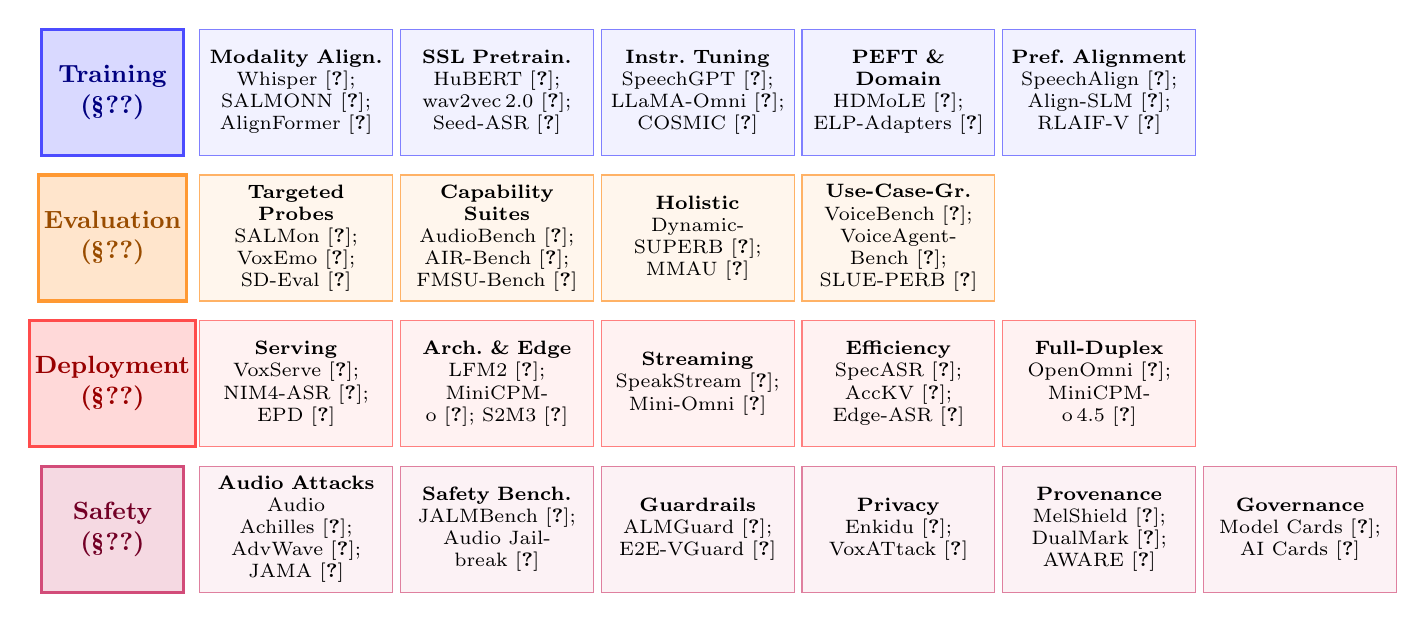
\begin{tikzpicture}[
  every node/.style={align=center, inner sep=2pt},
  stageT/.style={rectangle, draw=blue!70, very thick, fill=blue!15,
                 minimum width=1.8cm, minimum height=1.6cm,
                 font=\small\bfseries\color{blue!50!black}, align=center},
  stageE/.style={rectangle, draw=orange!80, very thick, fill=orange!20,
                 minimum width=1.8cm, minimum height=1.6cm,
                 font=\small\bfseries\color{orange!60!black}, align=center},
  stageD/.style={rectangle, draw=red!70, very thick, fill=red!15,
                 minimum width=1.8cm, minimum height=1.6cm,
                 font=\small\bfseries\color{red!60!black}, align=center},
  stageS/.style={rectangle, draw=purple!70, very thick, fill=purple!15,
                 minimum width=1.8cm, minimum height=1.6cm,
                 font=\small\bfseries\color{purple!60!black}, align=center},
  topicT/.style={rectangle, draw=blue!50, thin, fill=blue!5,
                 minimum width=2.45cm, minimum height=1.6cm,
                 text width=2.25cm, font=\scriptsize, anchor=west, align=center},
  topicE/.style={rectangle, draw=orange!60, thin, fill=orange!7,
                 minimum width=2.45cm, minimum height=1.6cm,
                 text width=2.25cm, font=\scriptsize, anchor=west, align=center},
  topicD/.style={rectangle, draw=red!50, thin, fill=red!5,
                 minimum width=2.45cm, minimum height=1.6cm,
                 text width=2.25cm, font=\scriptsize, anchor=west, align=center},
  topicS/.style={rectangle, draw=purple!50, thin, fill=purple!5,
                 minimum width=2.45cm, minimum height=1.6cm,
                 text width=2.25cm, font=\scriptsize, anchor=west, align=center}
]
% ROW 1: TRAINING
\node[stageT] (s1) at (0,0) {Training\\(\S\ref{sec:training_strategies})};
\node[topicT] (t1a) at (1.1,0)  {\textbf{Modality Align.}\\ Whisper~\cite{radford2023robust}; SALMONN~\cite{tang2023salmonn}; AlignFormer~\cite{fan2025alignformer}};
\node[topicT] (t1b) at (3.65,0) {\textbf{SSL Pretrain.}\\ HuBERT~\cite{hsu2021hubert}; wav2vec\,2.0~\cite{baevski2020wav2vec}; Seed-ASR~\cite{bai2024seed}};
\node[topicT] (t1c) at (6.20,0) {\textbf{Instr.~Tuning}\\ SpeechGPT~\cite{zhang2023speechgptempoweringlargelanguage}; LLaMA-Omni~\cite{fang2025llamaomniseamlessspeechinteraction}; COSMIC~\cite{pan2024cosmicdataefficientinstructiontuning}};
\node[topicT] (t1d) at (8.75,0) {\textbf{PEFT \& Domain}\\ HDMoLE~\cite{mu2025hdmolemixtureloraexperts}; ELP-Adapters~\cite{inoue2024elpadaptersparameterefficientadapter}};
\node[topicT] (t1e) at (11.30,0){\textbf{Pref.~Alignment}\\ SpeechAlign~\cite{zhang2024speechalignaligningspeechgeneration}; Align-SLM~\cite{lin2025alignslmtextlessspokenlanguage}; RLAIF-V~\cite{yu2024rlaifvopensourceaifeedback}};

% ROW 2: EVALUATION
\node[stageE] (s2) at (0,-1.85) {Evaluation\\(\S\ref{sec:evaluation_benchmarking})};
\node[topicE] at (1.1,-1.85)  {\textbf{Targeted Probes}\\ SALMon~\cite{maimon2024salmon}; VoxEmo~\cite{zhang2026voxemo}; SD-Eval~\cite{ao2024sdeval}};
\node[topicE] at (3.65,-1.85) {\textbf{Capability Suites}\\ AudioBench~\cite{wang2025audiobench}; AIR-Bench~\cite{yang2024airbench}; FMSU-Bench~\cite{li2026fmsubench}};
\node[topicE] at (6.20,-1.85) {\textbf{Holistic}\\ Dynamic-SUPERB~\cite{huang2024dynamicsuperb}; MMAU~\cite{sakshi2024mmau}};
\node[topicE] at (8.75,-1.85) {\textbf{Use-Case-Gr.}\\ VoiceBench~\cite{chen2024voicebench}; VoiceAgentBench~\cite{jain2025voiceagentbench}; SLUE-PERB~\cite{shon2023slue}};

% ROW 3: DEPLOYMENT
\node[stageD] (s3) at (0,-3.7) {Deployment\\(\S\ref{sec:deployment})};
\node[topicD] at (1.1,-3.7)  {\textbf{Serving}\\ VoxServe~\cite{kamahori2026voxserve}; NIM4-ASR~\cite{xie2026nim4asr}; EPD~\cite{singh2025epd}};
\node[topicD] at (3.65,-3.7) {\textbf{Arch.~\& Edge}\\ LFM2~\cite{amini2025lfm2}; MiniCPM-o~\cite{cui2026minicpmo}; S2M3~\cite{yoon2025s2m3}};
\node[topicD] at (6.20,-3.7) {\textbf{Streaming}\\ SpeakStream~\cite{bai2025speakstream}; Mini-Omni~\cite{xie2024miniomni}};
\node[topicD] at (8.75,-3.7) {\textbf{Efficiency}\\ SpecASR~\cite{wei2025specasr}; AccKV~\cite{jiang2025acckv}; Edge-ASR~\cite{feng2025edgeasr}};
\node[topicD] at (11.30,-3.7){\textbf{Full-Duplex}\\ OpenOmni~\cite{luo2025openomni}; MiniCPM-o\,4.5~\cite{cui2026minicpmo}};

% ROW 4: SAFETY
\node[stageS] (s4) at (0,-5.55) {Safety\\(\S\ref{sec:safety_privacy_governance})};
\node[topicS] at (1.1,-5.55)  {\textbf{Audio Attacks}\\ Audio Achilles~\cite{yang2024audioachillesheelred}; AdvWave~\cite{kang2024advwavestealthyadversarialjailbreak}; JAMA~\cite{krishnan2026optimizingmultimodaljailbreaksspoken}};
\node[topicS] at (3.65,-5.55) {\textbf{Safety Bench.}\\ JALMBench~\cite{peng2026jalmbenchbenchmarkingjailbreakvulnerabilities}; Audio Jailbreak~\cite{song2025audiojailbreakopencomprehensive}};
\node[topicS] at (6.20,-5.55) {\textbf{Guardrails}\\ ALMGuard~\cite{jin2025almguardsafetyshortcutsguardrails}; E2E-VGuard~\cite{zhang2025e2evguardadversarialpreventionproduction}};
\node[topicS] at (8.75,-5.55) {\textbf{Privacy}\\ Enkidu~\cite{feng2025enkiduuniversalfrequentialperturbation}; VoxATtack~\cite{aloradi2026voxattackmultimodalattackvoice}};
\node[topicS] at (11.30,-5.55){\textbf{Provenance}\\ MelShield~\cite{jin2026melshieldrobustmeldomainaudio}; DualMark~\cite{yang2025dualmarkidentifyingmodeltraining}; AWARE~\cite{pavlović2026awareaudiowatermarkingadversarial}};
\node[topicS] at (13.85,-5.55){\textbf{Governance}\\ Model Cards~\cite{Mitchell_2019}; AI Cards~\cite{golpayegani2024aicardsappliedframework}};
\end{tikzpicture}
\caption{Paper taxonomy of Speech LLM lifecycle research covered by
this survey. Representative methods and systems are grouped under the
four lifecycle stages introduced in
Figure~\ref{fig:lifecycle}. The taxonomy lists 2--3 representative
works per sub-topic to indicate scope; the full reference list and
benchmark coding are released as supplementary material.}
\label{fig:taxonomy}
\end{figure*}


Section~\ref{sec:background} introduces the speech-specific concepts
the survey relies on. Section~\ref{sec:training_strategies}
consolidates training strategies. Sections
\ref{sec:evaluation_benchmarking}, \ref{sec:deployment}, and
\ref{sec:safety_privacy_governance} develop the lifecycle audit for
evaluation, deployment, and safety. We close with open challenges
(Section~\ref{sec:future_directions}) and a synthesis
(Section~\ref{sec:conclusion}). The lifecycle map in
Figure~\ref{fig:lifecycle} traces these stages and the couplings the
survey emphasizes.

\begin{figure}[!t]
\centering
\begin{tikzpicture}[
  >=Stealth,
  every node/.style={font=\scriptsize},
  stage/.style={
    rectangle, draw=black!75, thick,
    minimum width=2.0cm, minimum height=0.7cm,
    align=center, fill=black!5
  },
  artifact/.style={font=\scriptsize\itshape, text=black!70, align=center},
  primary/.style={->, line width=0.9pt, draw=black!80},
  coupling/.style={->, line width=0.7pt, draw=black!55, dashed},
  arrowlabel/.style={font=\scriptsize, fill=white, inner sep=1.5pt}
]
% Four lifecycle stages at corners of a 4.5cm x 2.4cm rectangle (single-column fit).
\node[stage, fill=blue!15,   draw=blue!70]   (train)  at (0,2.4)  {\textbf{Training}};
\node[stage, fill=orange!20, draw=orange!80] (eval)   at (4.5,2.4){\textbf{Evaluation}};
\node[stage, fill=red!15,    draw=red!70]    (deploy) at (4.5,0)  {\textbf{Deployment}};
\node[stage, fill=purple!15, draw=purple!70] (safety) at (0,0)    {\textbf{Safety}};

% Artifacts placed OUTSIDE the wheel so they do not crowd the
% re-train / select-and-tune arrows in the interior.
\node[artifact, above=0.05cm of train]  {alignment, SSL, DPO/RLAIF};
\node[artifact, above=0.05cm of eval]   {construct, ecological,\\evaluator, operational validity};
\node[artifact, below=0.05cm of deploy] {streaming, serving,\\full-duplex, edge};
\node[artifact, below=0.05cm of safety] {audio jailbreak, voice cloning,\\privacy, provenance};

% Primary lifecycle arrows (clockwise) along the outside of the rectangle
\draw[primary] (train)  -- node[arrowlabel, midway] {validate}      (eval);
\draw[primary] (eval)   -- node[arrowlabel, midway] {select \& tune} (deploy);
\draw[primary] (deploy) -- node[arrowlabel, midway] {harden}        (safety);
\draw[primary] (safety) -- node[arrowlabel, midway] {re-train}      (train);

% One diagonal cross-stage coupling, bent slightly to avoid arrow labels
\draw[coupling] (train.south east) to[bend right=12]
  node[arrowlabel, pos=0.55] {training--deployment coupling}
  (deploy.north west);

% Legend as a single horizontal row below the wheel
\node[anchor=north, font=\tiny] at (2.25,-0.9) {
  \begin{tabular}{@{}c@{\hspace{2pt}}l@{\hspace{8pt}}c@{\hspace{2pt}}l@{}}
    \tikz[baseline=-0.6ex] \draw[primary] (0,0) -- (0.35,0); & Primary &
    \tikz[baseline=-0.6ex] \draw[coupling] (0,0) -- (0.35,0); & Coupling \\
  \end{tabular}
};
\end{tikzpicture}
\caption{The Speech LLM lifecycle as a coupled system. Solid arrows
trace the conventional cycle from training through evaluation,
deployment, and safety, with re-training closing the loop. The dashed
diagonal highlights the survey's central claim that the cycle is not
purely sequential: training choices shape deployment feasibility,
and the consequences of evaluation, deployment, and safety choices
feed back through re-training.}
\label{fig:lifecycle}
\end{figure}

To make the cross-stage couplings concrete, Table~\ref{tab:coupling_evidence}
records five examples where a training, evaluation, or deployment choice
documented in the literature produced a visible consequence in a
downstream stage.

\begin{table*}[t]
\caption{Concrete cross-stage couplings observed in the literature
covered by this survey. Each row links a specific upstream decision to
a documented downstream consequence, illustrating that the four
lifecycle stages are not independent.}
\label{tab:coupling_evidence}
\centering
\footnotesize
\begin{tabularx}{\textwidth}{|p{0.13\textwidth}|X|X|X|}
\hline
\textbf{Upstream stage} & \textbf{Decision / observation} &
\textbf{Downstream stage affected} & \textbf{Documented consequence} \\
\hline
Training &
Whisper-style weakly supervised pretraining emphasizes transcription
quality \cite{radford2023robust}. &
Evaluation &
Benchmarks inherit ASR-centric metrics; paralinguistic and prosodic
validity are under-measured (Section~\ref{subsec:eval_coverage}). \\
\hline
Training &
Adapter / Q-Former bridge between speech encoder and language model
\cite{tang2023salmonn,fan2025alignformer}. &
Deployment &
Bridge layer adds latency; full-duplex stacks must redesign streaming
boundary (Section~\ref{sec:deployment}). \\
\hline
Evaluation &
Multilinguality coverage is fragmented across incompatible metrics
\cite{liu2025seallmsaudio,papi2025hearing2translate}. &
Deployment &
Practitioners cannot rank multilingual systems for production without
re-running on a target language slice (Section~\ref{sec:deployment}). \\
\hline
Evaluation &
LLM-as-judge protocols underlie open-ended scoring with only moderate
human correlation \cite{ao2024sdeval,zheng2023judging}. &
Safety &
Judge-based reward signals can miss unsafe prosody or jailbreaks
triggered by acoustic content (Section~\ref{sec:safety_privacy_governance}). \\
\hline
Deployment &
Quantization and KV-cache pruning are applied for edge feasibility
\cite{xie2024miniomni}. &
Safety &
Downstream safety classifiers and watermark detectors can degrade
under aggressive compression
(Section~\ref{sec:safety_privacy_governance}). \\
\hline
\end{tabularx}
\end{table*}
\FloatBarrier